\documentclass[14pt,final]{report}
\usepackage{graphicx}
\usepackage{wrapfig}

\usepackage{caption}
% \usepackage[english,russian]{babel}

% TODO: Do something 
% https://www.overleaf.com/read/fkzbbcxxrxvz
% This was edited locally
% And this was edited on the server

% \RequirePackage{polyglossia}
% \setotherlanguage{english}
% \setdefaultlanguage{russian}

\RequirePackage[times,firacode,a4paper,microtyping,732,smalltitles,listbib,lmmath]{subook}
% \RequirePackage[times,firacode,a4paper,microtyping,handbook,smalltitles,listbib]{subook}
\RequirePackage{tabularx}
% \RequirePackage{grphicx}
\graphicspath{{pics/}}

% \usepackage{showframe}

% pygmetize
\RequirePackage{minted}
\usemintedstyle{tango} % bw

% \setmainfont{Times New Roman}

\begin{document}
\thispagestyle{empty}
\begin{center}
МИНИСТЕРСТВО ОБРАЗОВАНИЯ И НАУКИ РОССИЙСКОЙ ФЕДЕРАЦИИ

Федеральное государственное бюджетное образовательное учреждение высшего образования

«ИРКУТСКИЙ  ГОСУДАРСТВЕННЫЙ УНИВЕРСИТЕТ»\\
(ФГБОУ ВО «ИГУ»)
\end{center}
\vfill % \vfil \vfill \vfilll

\noindent\begin{tabularx}{\textwidth} {
  >{\raggedright\arraybackslash}X
  >{\raggedright\arraybackslash}X }
Институт математики и информационных технологий
&
Информационных технологий
\end{tabularx}

\vfill
\begin{center}
  \textbf{ОТЧЕТ}
\vspace{1em}

о курсовой работе по курсу <<Разработка WEB-приложений>>

{\bf Проектирование мессенджера}

\end{center}
\vfill

\noindent\begin{tabularx}{\textwidth} {
  >{\raggedright\arraybackslash}X
  >{\raggedright}X }
&

Студента 3 курса группы 2371\\
Парунова Ильи Владимировича\\
Направление\;: 02.03.02~--~Фундаментальная информатика и информационные технологии\\[2em]

Руководитель:\\
доцент\\
Черкашин Евгений Александрович\\[2em]

Курсовая работа защищена с оценкой\\[1em] \underline{\hspace{3cm}}
\end{tabularx}
\vfill
\begin{center}
  Иркутск -- 2021
\end{center}
\clearpage

\tableofcontents

\chapter*{ВВЕДЕНИЕ}

\label{chap:intro}
За последние несколько лет популярность мессенджеров взлетела: ещё недавно пользователям вполне хватало обычных смс и переписки в контакте, а сейчас многие не представляют свою жизнь без любимого приложения. Поэтому, в качестве учебного проекта, было принято решение создать веб-мессенджер.\\
\\ \noindent
\textbf{Актуальность:} использование мессенджеров обусловлено желанием пользователей мгновенно доставить сообщение, и в кратчайшие сроки получить ответ с легкой доступностью к его написанию и прочтению.\\
\textbf{Объектом автоматизации} является мессенджер.\\
\textbf{Предмет автоматизации} - разработка программной системы на основе React JS.\\
Функциями программного продукта в первую очередь являются отправка и получение сообщений, с возможностью изменения некоторых параметров пользовательского профиля таких как: фотография профиля, имя профиля.\\
\textbf{Целью} данной работы является написание веб-приложения представляющее собой мессенджер. Для достижения поставленной цели решены
следующие задачи:\\
\begin{enumerate}
    \item Изучена предметная область проекта;
    \item Выработаны требования к ИС;
    \item Создан общий дизайн ИС;
    \item Разработана реляционная база данных;
    \item Реализованы функции клиентской части ИС;
\end{enumerate}

\chapter{Основы Frontend разработки с помощью библиотеки React и Fetch API}

\section{Требования к продукту}
К программному продукту предъявляются следующие требования:

\begin{enumerate}
    \item Должна быть возможность регистрации и авторизации пользователей;
    \item Должна быть возможность отправки сообщений;
    \item Должна присутствовать возможность добавлять зарегистрированных пользователей в список контактов;
\end{enumerate}

\section{Архитектура приложения}
Разработка состояла из двух частей: разработка серверной части и разработка
клиентской части.\\
Серверная часть и клиентская части программы находятся на разных машинах, это означает, что получившаяся система обладает клиент-серверной архитектурой (рис. \ref{architect}).\\
При клиент-серверной архитектуре серверная часть программы ожидает от клиентской части
запросы и предоставляют им свои ресурсы в виде полученной с базы данных информации.

\begin{figure}[h]
\centering
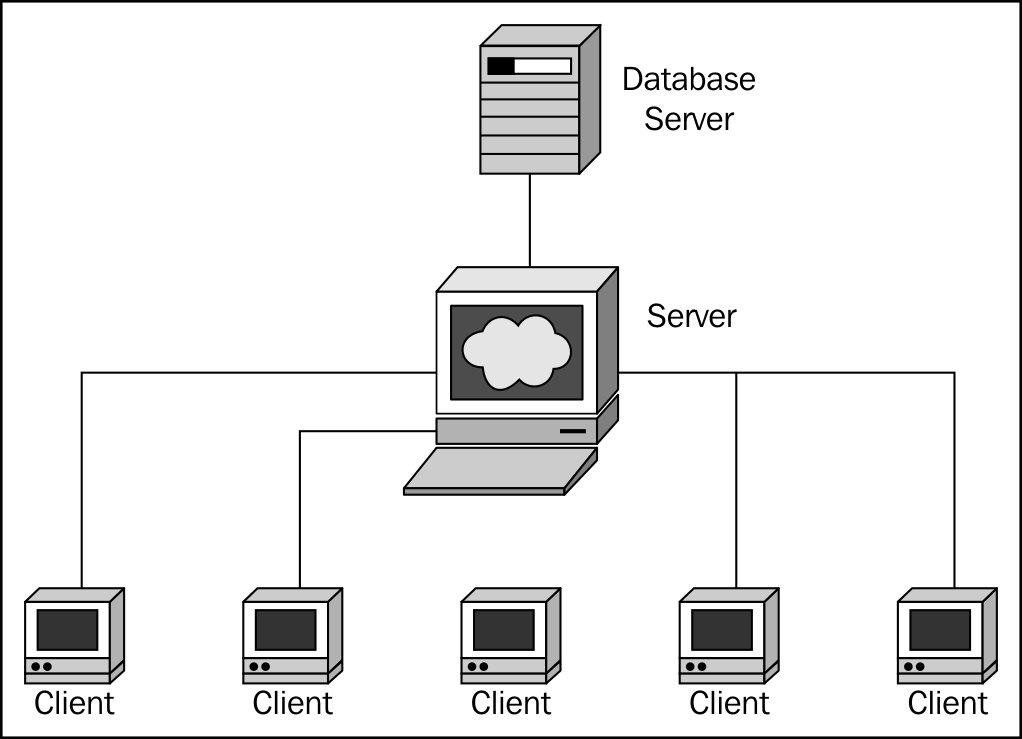
\includegraphics[scale=0.4 ]{architecture.jpg}
\caption{Клиент-серверная архитектура}
\label{architect}
\end{figure}

\newpage
\section{Среда разработки и библиотеки}
Средой разработки была выбрана JetBrains WebStorm. WebStorm — интегрированная среда разработки на JavaScript, CSS & HTML от компании JetBrains. WebStorm обеспечивает автодополнение, анализ кода на лету, навигацию по коду, рефакторинг, отладку, интеграцию с системами управления версиями, и самое важное для нас - это Поддержка React и JSX.\\ 
\\
В качестве инструмента для осуществления взаимодействия серверной и клиентской части использовался Fetch API. Fetch API  предоставляет интерфейс для получения ресурсов. Fetch – это новый API, основанный на промисах. В свою очередь объект Promise представляет возможное завершение или сбой асинхронной операции и ее результирующее значение. Работая с промисами-обещаниями, мы должны знать, каково его текущее состояние, т.к. у этого объекта есть три состояния: Ожидание (Pending), Выполнено (Fulfilled ) и Отклонено (Rejected). Fetch поддерживается всеми современными браузерами, поэтому использовать его действительно несложно.
\\
\\
Со стороны клиентской части использовались следующие библиотеки:
\begin{enumerate}
    \item React;
    \item React-redux;
    \item Redux-thunk;
\end{enumerate}
React \cite{vuruh} — это JavaScript-библиотека с открытым исходным кодом для разработки пользовательских интерфейсов. Цель React — предоставить высокую скорость, простоту разработки приложений, а также минимизировать возникающие. Достигается это за счет того, что используются так называемые компоненты (автономные логические фрагменты кода, которые описывают часть интерфейса, которые объединяются для создания полноценного интерфейса).

Зачастую в связке с React используется библиотека Redux. Она также имеет откртый исходный код, но предназначена для управления состоянием приложения.

Для связки React и Redux \cite{banks} используется библиотека React-redux.Также была использована еще одна полезная библиотека — Redux Thunk \cite{thomas}. Она позволяет вызывать создателей действий, которые возвращают функцию вместо объекта действия. Другими словами это какая-то функция, которая берёт текущее состояние, текущее действие и что-то делает с этим.

\chapter{Реализация React приложения}

На основе предоставленной серверной части и реляционной базе данных (рис. \ref{database}), были реализованы основные функции клиентской части. \\
Основные из них:
\begin{enumerate}
    \item Регистрация и авторизация;
    \item Отправка сообщений;
    \item Добавление других пользователей в список контактов;
\end{enumerate}

\begin{figure}[h]
\centering
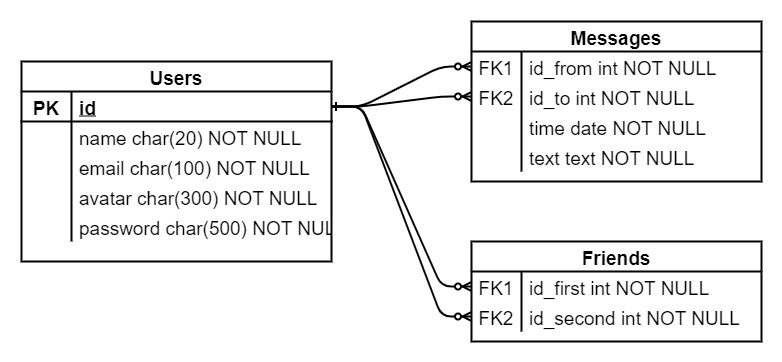
\includegraphics[scale=0.4 ]{5CzTRFz5alk.jpg}
\caption{Реляционная база данных}
\label{database}
\end{figure}
В процессе разработки часто будут использоваться reducers \cite{mardan} (редьюсеры), поэтому обозначим
что это. Как мы знаем в Redux все состояние приложения хранится в виде единственного объекта, и поэтому для удобства изменения конкретных полей состояния и были придуманы редьюсеры, то есть редьюсеры это функции, которые меняют состояния и возвращают его в измененном виде. Но как они понимают, что именно нужно изменить? Здесь на помощь приходят dispatchers (диспетчеры), диспетчеры передают в редьюсеры информацию о том какой тип действия должен быть применен, и передают объект, в котором хранится наше измененное состояние. Редьюсеры реализованы внутри себя оператором switch-case, в котором кейсы будут соответствовать
типам действий. Также для ускорения разработки и минимизации ошибок были введены action-creators (создатели действия), это функция, которая принимается диспетчером, но уже содержит в себе тип действия, и остается только передать измененное состояние. \\
\\
Рассмотрим как пример редьюсер авторизации пользователя (лист. \ref{auth-reducer})
\newpage
\begin{listing}[!h]
\begin{minted}{js}
let defaultState = {
        auth: false
}

const AUTH_USER = "AUTH_USER";

export const authUserReducer = (state = defaultState, action) => {
    switch (action.type) {
        case AUTH_USER:
            return {...state, auth: true}
        default:
            return state;
    }
}

export const authUserAction = (data) => ({type: AUTH_USER, data: data})
\end{minted}
\caption{Редьюсер авторизации}
\label{auth-reducer}
\end{listing}

\subsection{Регистрация и авторизация}
Для реализации функций регистрации и авторизации используется компонента, в которой при нажатии на некоторые объекты внутри, вызываются определенные функции.
Функции в свою очередь выполняют запросы к серверу и при надобности изменяют состояния.
Функция регистрации пользователя по введенным в форму данным посылает серверу post запрос, после чего на серверной части в базу данных вносится новая запись.\\
При выполнении функции авторизации используется не только put-запрос к серверу, но и
меняется состояние при помощи reducer. При выполнении функции вызывается dispatch
и ему передается функция, возвращающая action <<AUTH\_USER>> и параметры, введенные в форму
авторизации. Для обработки нового события в authUserReducer определяется соответствующий кейс, который для этого события устанавливает значение текущего пользователя и помечает логическую переменную auth как истинную. Таким образом, при вводе данных в форму и нажатии кнопки <<войти>>, произойдет событие <<AUTH\_USER>>, которое будет передано диспетчеру, а тот в свою очередь отправит эти данные редюсеру, запоминающему текущего пользователя.
Затем подгружалась уже имеющаяся информация о пользователе (имя, фотография профиля, уже начатые диалоги). Для этого всего вызывалиь соответствующие диспетчеры, в функции авторизации.\\
Реализация функций приведена в прил. \ref{search}, \ref{changePhoto}, \ref{changeName}\\
Релизация соответствующих редьюсеров приведена в прил. \ref{searchReducer}\\ \ref{changePhotoReducer}, \ref{changeNameReducer}\\
Функция регистрации (прил. \ref{register}) и функция авторизации (прил. \ref{auth})


\subsection{Отправка сообщений}
Для того, чтобы пользователи могли отправлять сообщения, в соответствующей компоненте была реализована функция, которая выполнялась при нажатии на кнопку отправки сообщения. Но для начала в диалог должна была подгрузиться уже имеющаяся переписка с пользователем, если она осуществлялась. Для этого при клике на какой-либо диалог вызывалась функция loadMessages, которая отправляла post запрос на сервер с идентификаторами текущего пользователя, и того, с кем диалог мы хотим открыть, и в ответе получали объект со всеми имеющимися сообщениями. После чего ответ с сервера отправлялся в соответствующий редьюсер (реализация приведена в прил. \ref{sendReducer}) и дальше редьюсер обрабатывал полученный ответ.
Функция отправки сообщения (лист. \ref{send})


\subsection{Добавление других пользователей в список контактов}
Для того, чтобы пользователь мог добавлять в список контактов другого пользователя была реализована функция findPerson, которая вызывалась при нажатии кнопки поиска. В некую форму вводился email пользователя по которому он был зарегистрирован, если пользователь был найден, то он успешно добавлялся в список контактов, иначе выводилось предупреждение о некорректности введенных данных. В функции findPerson отправлялся post запрос на сервер с введенным в форму email'ом, после чего получала ответ и с помощью диспетера отдавала его на обработку в редьюсер Реализация приведена в прил. \ref{searchReducer}\\
Функция добавления контакта (лист. \ref{search})
\\
Также стоит отметить, что по аналогичной схеме были реализованы смена имени и фотографии профиля текущего пользователя. Реализация приведена в прил.\\ Реализация функций приведена в прил. \ref{search}, \ref{changePhoto}, \ref{changeName}\\
Релизация соответствующих редьюсеров приведена в прил. \ref{searchReducer}\\


\chapter*{ЗАКЛЮЧЕНИЕ}
По итогу проделанной работы было разработано веб-приложение представляющее из себя
простой мессенджер, и позволяющий пользователям:
\begin{enumerate}
    \item Регистрироваться и авторизоваться в системе;
    \item Отправлять сообщения;
    \item Добавление новых пользователей в список контактов;
    \item Изменять имя и аватарку в профиле;
\end{enumerate}
В частности использование библиотек React и Redux позволило достаточно продуктивно производить реализацию клиентской части приложения, а также взаимодействия клиента с серверной частью.\\
Также для совершенствования приложения можно реализовать следующие функции:
\begin{itemize}
    \item Получение сообщения без необходимости перезагрузки всего диалога
    \item Возможность отправки файлов (картинок, аудио и др.)
    \item Возможность удаления сообщений и контактов
    \item Отправку уведомлений в браузере
    \item Зашифрованная передача сообщений
    \item Наличие отдельных таблиц в БД для хранения персональных данных
\end{itemize}




\begin{thebibliography}{99}
\bibitem{thomas} М~.Т.~Томас. React в действии. М\;~Питер. 2019. 368~с.
\bibitem{vuruh} Р~.Вирух.Путь к изучению React. М\;~Питер. 2018. 231~с.
\bibitem{banks} А~.Бэнкс. Е~.Порселло. React и Redux: функциональная веб-разработка. М\;~Питер. 2018. 336~с.
\bibitem{mardan} А~.Мардан. React быстро. Веб-приложения на React, JSX, Redux и GraphQL. М\;~Питер. 2019. 560~с.
\end{thebibliography}

\appendices

\chapter{ПРИЛОЖЕНИЕ А Исходный код}
\begin{listing}[!h]
\begin{minted}{js}
    const reg = (mail, password, name) => {
        if (mail.length < 2 || password.length < 2 || name.length < 2) return

        let newUser = {
            email: mail,
            name: name,
            password: password,
        }
        fetch('http://127.0.0.1:5000//register', {
            method: 'post',
            headers: {
                "Access-Control-Allow-Origin": "*",
                "Access-Control-Allow-Methods": "POST, GET, PUT",
                "Access-Control-Allow-Headers": "Content-Type, Access-Control-Allow-Headers, Authorization, X-Requested-With",
                'accept': 'application/json',
                'content-type': 'application/json'
            },
            body: JSON.stringify(newUser)
        })
            .then((status) => {
                alert('Статус регистрации ' + (status.ok ? 'Успешно' : 'Не удалось'))
            })
            .catch(function (error) {
                console.log('Request failed', error);
            });
        
        setNewPass('')
        setNewLog('')
        setNewName('')
    }
\end{minted}
\caption{Функция регистрации пользователя}
\label{register}
\end{listing}

\begin{listing}[!h]
\begin{minted}{js}
  const Auth = () => {
    const navigate = useNavigate();
    const dispatch = useDispatch();
    const [newLog, setNewLog] = useState('')
    const [newPass, setNewPass] = useState('')
    const [newName, setNewName] = useState('')

    const enter = (email, password) => {
        const obj = {
            email: email,
            password: password
        }
        
        fetch('http://127.0.0.1:5000//login', {
            method: 'post',
            headers: {
                'Access-Control-Allow-Origin': '*',
                'Access-Control-Allow-Methods': 'GET, POST, PUT, DELETE, OPTIONS',
                'Accept': 'application/json',
                'Content-Type': 'application/json'
            },
            body: JSON.stringify(obj)
        })
            .then(response => response.json())
            .then((status) => {
                if (status.user) {
                    dispatch(authUserAction({data: true}))

                    const id = status.user.id;
                    const name = status.user.name;
                    const avatar = status.user.avatar;
                    const friends = status.friends;

                    dispatch(changeNameAction({name, id}));
                    dispatch(changePhotoAction({avatar, id}))
                    dispatch(findDialogsAction(friends))

                    navigate('/main');
                } else {
                    alert("Неправильный логин или пароль")
                }
            })
            .catch((error) => {
                console.log(error)
            });
    }  
\end{minted}
\caption{функция авторизации}
\label{auth}
\end{listing}

\begin{listing}[!h]
\begin{minted}{js}
let defaultState = {
        auth: false
}

const AUTH_USER = "AUTH_USER";

export const authUserReducer = (state = defaultState, action) => {
    switch (action.type) {
        case AUTH_USER:
            return {...state, auth: true}
        default:
            return state;
    }
}

export const authUserAction = (data) => ({type: AUTH_USER, data: data})
\end{minted}
\caption{Редьюсер авторизации}
\label{auth-reducer}
\end{listing}

\begin{listing}[!h]
\begin{minted}{js}
    const sendMessage = (text) => {

        const obj = {
            id_from: myId,
            id_to: idTo,
            text: text,
        }

        fetch('http://127.0.0.1:5000//send_message', {
            method: 'post',
            headers: {
                'Access-Control-Allow-Origin': '*',
                'Access-Control-Allow-Methods': 'GET, POST, PUT, DELETE, OPTIONS',
                'Accept': 'application/json',
                'Content-Type': 'application/json'
            },
            body: JSON.stringify(obj)
        })
            .then(response => {
                if (response.ok) {
                    dispatch(sendMessageAction(obj))
                }})
            .catch((error) => {
                console.log(error)
            });

        setNewMessage('')
    }
\end{minted}
\caption{Функция отправки сообщения}
\label{send}
\end{listing}

\begin{listing}[!h]
\begin{minted}{js}
const defaultState = {
        messages: [],
        id: 0
}

const SEND_MESSAGE = 'SEND_MESSAGE'
const FIND_MESSAGE = 'FIND_MESSAGE'

export const sendMessageReducer = (state = defaultState, action) => {
    switch (action.type) {
        case SEND_MESSAGE:
            if (action.data.text.length !== 0){
                return {...state, messages: [...state.messages, action.data]}
            }
            return state
        case FIND_MESSAGE:
            return {...state, messages:  action.messages, id: action.id}
        default:
            return state
    }
}

export const sendMessageAction = (data) => ({type: SEND_MESSAGE, data: data})
export const findMessageAction = (data) => ({type: FIND_MESSAGE, messages: data.messages, id: data.id})
\end{minted}
\caption{Функция отправки сообщения}
\label{sendReducer}
\end{listing}

\begin{listing}[!h]
\begin{minted}{js}
    const findPerson = (email) => {
        if (email.length < 2) {
            return
        }
        let obj = {
            id: userId,
            email: email
        }
        
        fetch('http://127.0.0.1:5000//get_user', {
            method: 'post',
            headers: {
                'Access-Control-Allow-Origin': '*',
                'Access-Control-Allow-Methods': 'GET, POST, PUT, DELETE, OPTIONS',
                'Accept': 'application/json',
                'Content-Type': 'application/json'
            },
            body: JSON.stringify(obj)
        })
            .then(response => response.json())
            .then((status) => {
                    if(status.id){
                        const id = status.id;
                        const name = status.name;
                        const avatar = status.avatar;

                        let newDialog = {
                            id: id,
                            name: name,
                            avatar: avatar
                        }

                        dispatch(addDialogAction(newDialog))
                    }
            })
            .catch((error) => {
                console.log(error)
            });

        setValue('');
    }
\end{minted}
\caption{Функция поиска}
\label{search}
\end{listing}

\begin{listing}[!h]
\begin{minted}{js}
let defaultState = {
        dialogsPage: []
}

const ADD_DIALOG = "ADD_DIALOG";
const FIND_DIALOG = "FIND_DIALOG";

export const addDialogReducer = (state = defaultState, action) => {
    switch (action.type) {
        case ADD_DIALOG:
            let userId = action.data.id
            for (let i=0; i < state.dialogsPage.length; i++) {
                if (state.dialogsPage[i].id === userId){
                    return state
                }
            }
            return {...state, dialogsPage: [...state.dialogsPage, action.data]}
        case FIND_DIALOG:
            return {...state, dialogsPage: action.data}
        default:
            return state;
    }
}

export const addDialogAction = (data) => ({type: ADD_DIALOG, data: data})
export const findDialogsAction = (data) => ({type: FIND_DIALOG, data: data})
\end{minted}
\caption{Редьюсер для поиска}
\label{searchReducer}
\end{listing}

\begin{listing}[!h]
\begin{minted}{js}
    function changePhoto(newPhotoLink){

        if (newPhotoLink.length < 2){
            return
        }

        const obj = {
            id: changePhotoId,
            avatar: newPhotoLink
        }

        fetch('http://127.0.0.1:5000//renew_avatar', {
            method: 'post',
            headers: {
                'Access-Control-Allow-Origin': '*',
                'Access-Control-Allow-Methods': 'GET, POST, PUT, DELETE, OPTIONS',
                'Accept': 'application/json',
                'Content-Type': 'application/json'
            },
            body: JSON.stringify(obj)
        })
            .then(response => {
                if (response.ok){
                    dispatch(changePhotoAction(obj));
                }
            })
            .catch((error) => {
                console.log(error)
            });

        setNewPhotoLink('')
    }
\end{minted}
\caption{Функция смены фотографии}
\label{changePhoto}
\end{listing}

\begin{listing}[!h]
\begin{minted}{js}
let defaultState = {
    userId: 0,
    photoLink: ''
}

const CHANGE_PHOTO = 'CHANGE_PHOTO';

export const changePhotoReducer = (state = defaultState, action) => {
    switch (action.type) {
        case CHANGE_PHOTO:
            return {...state, userId: action.id, photoLink: action.link}
        default:
            return state
    }
}


export const changePhotoAction = (data) => {
    return {type: CHANGE_PHOTO, link: data.avatar, id: data.id}
}

\end{minted}
\caption{Редьюсер для смены фотографии}
\label{changePhotoReducer}
\end{listing}

\begin{listing}[!h]
\begin{minted}{js}
function changeName(newName) {

        if (newName.length < 2){
            return
        }

        const obj = {
            id: changeNameId,
            name: newName
        }

        fetch('http://127.0.0.1:5000//renew_name', {
            method: 'post',
            headers: {
                'Access-Control-Allow-Origin': '*',
                'Access-Control-Allow-Methods': 'GET, POST, PUT, DELETE, OPTIONS',
                'Accept': 'application/json',
                'Content-Type': 'application/json'
            },
            body: JSON.stringify(obj)
        })
            .then(response => {
                if (response.ok){
                    dispatch(changeNameAction(obj))
                }
            })
            .catch((error) => {
                console.log(error)
            });

        setNewName('')
    }
\end{minted}
\caption{Функция смены имени}
\label{changeName}
\end{listing}

\begin{listing}[!h]
\begin{minted}{js}
let defaultState = {
    userId: 0,
    userName: ''
}

const CHANGE_NAME = 'CHANGE_NAME';

export const changeNameReducer = (state = defaultState, action) => {
    switch (action.type) {
        case CHANGE_NAME:
            return {...state, userName: action.name, userId: action.id}
        default:
            return state
    }
}

export const changeNameAction = (data) => {
    return {type: CHANGE_NAME, name: data.name, id: data.id}
}
\end{minted}
\caption{Редьюсер для смены имени}
\label{changeNameReducer}
\end{listing}




\end{document}

%%% Local Variables:
%%% mode: latex
%%% TeX-master: t
%%% End:
